\documentclass[10pt]{article}

%%%%    FORMATTING    %%%%
\usepackage{url}
\usepackage[utf8]{inputenc}
\usepackage{amsmath}
\usepackage{amssymb}
%\usepackage{wasysym}
\usepackage[dvipsnames]{xcolor}
\usepackage[version=4]{mhchem}
\usepackage{verbatim}
\usepackage{graphicx}
\usepackage[export]{adjustbox}
\usepackage[margin=1in]{geometry}
\usepackage[titletoc, title]{appendix}
\usepackage{hyperref}
\hypersetup{
    colorlinks = true,
    citecolor = red,
    linkcolor = blue,
    urlcolor = black,
}
%For code in appendix
\usepackage{listings}
\usepackage{color}
\definecolor{mygreen}{rgb}{0,0.6,0}
\definecolor{mygray}{rgb}{0.5,0.5,0.5}
\definecolor{mymauve}{rgb}{0.58,0,0.82}
\lstset{ %
  backgroundcolor=\color{white},   % choose the background color
  basicstyle=\footnotesize,        % size of fonts used for the code
  breaklines=true,                 % automatic line breaking only at whitespace
  captionpos=b,                    % sets the caption-position to bottom
  commentstyle=\color{mygreen},    % comment style
  escapeinside={\%*}{*)},          % if you want to add LaTeX within your code
  keywordstyle=\color{blue},       % keyword style
  stringstyle=\color{mymauve},     % string literal style
  frame = tb,
  numbers = left
}




\title{nEXO OD FLUKA Simulations Manual}
\author{Regan Ross}

%%%%    BEGIN DOCUMENT    %%%
\begin{document}

%%%%    Title Page    %%%
\begin{titlepage}
    \maketitle
    \vspace{4cm}
    \centering
    % \includegraphics*[scale=0.5, frame]{./figs/muons_det.png}
\end{titlepage}

\begin{abstract}
    This document is intented to provide insight into the functioning of the nEXO FLUKA simulations and justifications for choices made in their design. Further, this work should provide a near comprehensive baseline for anyone willing to replicate similar cosmogenic studies for the nEXO collaboration, or even another. FLUKA can be a daunting software to work with given it is written in FORTRAN77, has sparse documentation, and whose source code, without a specific licence, is veiled to the user. However, this proprietary simulation program is fast and rich with built-in features that have been used extensively for decades. Moreover, it is particularly useful for the case of studying cosmogenic muons at several hundred GeV energies and their secondaries. This document will provide an overview and explanation of the FLUKA features enabled for the specific nEXO Outer Detector (OD) case and an overview of the additional user routines, scripts, and containerization procedures that are all ancilliary to the base simulations (but required to run the simulations on the SDF cluster and perform the more in-depth analyses required by our questions).
\end{abstract}


\vspace{1.5cm}
\listoffigures

\newpage
\tableofcontents

\break
%%%%%%%%%%%%%%%%%%%%%%%%%%%%%%%%%%%%%%
%                                   %
%%%%    The FLUKA Input File     %%%%
%                                   %
%%%%%%%%%%%%%%%%%%%%%%%%%%%%%%%%%%%%%%
\part*{The FLUKA Input File (`.inp')}
\section{Introduction}
    \paragraph{}
    The input file is exactly as it is named— it is the De facto interface between the user and the FLUKA binaries. It contains, among other things, the entire physical configuration of the media through which the particles are transported, the defining characteristics of the impinging beam, options for enabling particular physical processes, definitions of materials, and cards to deploy default FLUKA scoring methods. It is a human-readable ascii file with a very specific format. Each input card in the input file must not contain more than 8 fields each of which has a character limit. This is due (presumably) to constraints in the early development of FLUKA. Programmed in FORTRAN77 which imposes constrains on the length of statements which, in the early days, were written into computers (with very little memory) using paper punch cards. Now, this formatting is an annoying anachronism but it probably does still keep the program slim and fast. Generally though, a user need not worry about writing the input file directly, as there is a great GUI interface to FLUKA called \textit{flair} which, by the way, is open source and contains all the possible input options. The next section will overview the specific components of the nEXO OD input file and the functions they serve.


\section{The nEXO OD Input File}

\subsection{Geometry}
\paragraph{}
Arguably the most important parts of the input file are the cards defining the configuration space— namely the detector and media with respect to the cartesian coordinate system. In FLUKA this is known as the \textit{geometry}. The geometry section of the input card is demarcated by \textbf{GEOBEGIN} and \textbf{GEOEND} cards. Between these two cards are first, cards for various \textit{bodies} which are basic 2D and 3D geometric surfaces and second, cards for \textit{regions} whose bounds are defined by combinations of geometric \textit{bodies}. For instance, a triplet of bodies could be a cylinder whose axis lies on the $z$-axis, and two planes lying parallel the $x-y$ plane at different $z$s. A region defined by these bodies could be the 3D cylindrical volume made by the cylinder body capped off on either end by the two planes. This is exactly the type of region representing the nEXO OD and the nEXO TPC. 

\begin{figure}[h]
    \begin{center}
    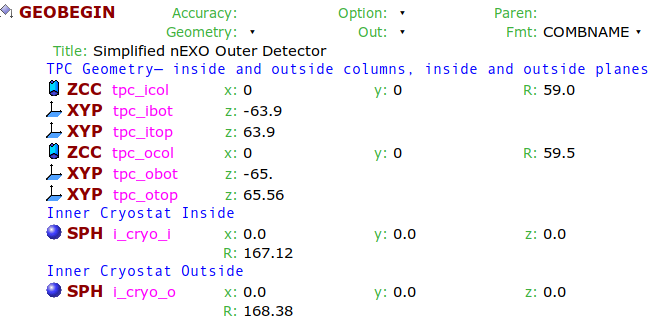
\includegraphics[scale=0.5]{figures/geometry_1.png}
    \caption{An example of the geometry body declarations in the input file}
    \label{fig:geometry1}
    \end{center}
\end{figure}

\paragraph{}
Figure \ref{fig:geometry1} shows the first part of the geometry declarations in the nEXO input file. We see the first card is the \textbf{GEOBEGIN} with the argument \textit{fmt} set to COMBNAME. This tells the FLUKA binaries how to read in the following geometry cards. This is not particularly important. This seems to be the default mode. Text in \textcolor{blue}{blue} indicates a comment (equivalent to a FORTRAN77 comment in the input file) and body variable names are in \textcolor{magenta}{pink} and are limited to lengths of 8 characters. The names or types of cards are fully capitalized and in \textcolor{Maroon}{maroon}. The argument names for each card are written in \textcolor{ForestGreen}{green} and the arguments follow with an 8 character length limit. These colour conventions hold for every other type of input card. Each card can have many arguments, but generally, not all are necessary. In the geometry body cards however, each argument is provided as these arguments are all necessary to uniquely define their respective geometric body. For instance, there is a body called \textcolor{magenta}{i\_cryo\_i} defined with a \textcolor{Maroon}{SPH} card. The name is intented to be shorthand for ``inner cryostat inside'' and, being a sphere, requires a radius and three coordinates for its location in space. There are many choices for bodies in FLUKA, each of which fairly simple to define.

\paragraph{}
Regions, as previously discussed, are created with logical combinations of bodies. Imagine the bodies defining surfaces in 3D, and the regions being the volumes they surround. Following the set of cards defining the bodies, there is an \textbf{END} card, then the region cards as shown in figure \ref{fig:geometry2}, finally there is the \textbf{GEOEND} card. Each region must be assigned \textbf{one} material— we'll get to material assignments later. For example, the region inside the nEXO OD that is full of water would be defined by the OD inside body minus the outer cryostat outside body leaving the configuration of a cylinder with a spherical hole in its volume— the entirety of this region is to be water. 

\begin{figure}[h]
    \begin{center}
    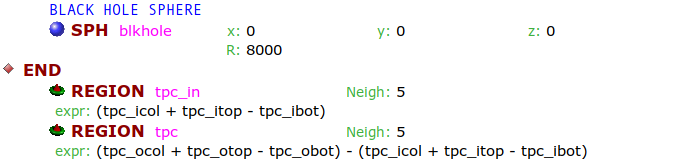
\includegraphics[scale=0.5]{figures/geometry_2.png}
    \caption{An example of the geometry region declarations in the input file}
    \label{fig:geometry2}
    \end{center}
\end{figure}

\paragraph{}
Looking at figure \ref{fig:geometry2}, we see the final body declaration followed by the first few region declarations in the nEXO input file. The final body here is important— each FLUKA configuration defines its physical boundaries by assigning material \textit{blackhole} to its outermost surface- hence the name of the sphere. The first region we have defined is \textcolor{magenta}{tpc\_in} will be the inside of the TPC cylinder— the part filled with liquid xenon. While no number is assigned by the user to the region, FLUKA assigns it number 1 as it is the first defined- this will be important later. The construction of the region is in the \textcolor{ForestGreen}{expr} argument given by ``(tpc\_icol $+$ tpc\_itop $-$ tpc\_ibot)''. We first have \textit{tpc\_icol} which is the inside cylinder (along $z$) of the TPC which alone is unbound and spans the entire $z$-axis. To the cylinder we add \textit{tpc\_itop} (xy-plane) which sets the upper bound, and subtract \textit{tpc\_ibot} (xy-plane) which sets the lower bound. This process is similar for all other region declarations. Unfortunately, one may not reference regions by name in region expressions, only bodies; hence the following region declaration of the \textcolor{magenta}{tpc} which is intended to be the material composing the TPC. The \textcolor{ForestGreen}{Neigh} argument is an integer which defines ``neighbourhoods'' relating regions to each other. This can perhaps be deployed for larger, more complex geometries but given the simplicity of the nEXO OD geometry and the lack of thorough documentation of this feature, it has been set to the default value of 5 for each region. Once more, the \textbf{GEOEND} card (not shown) brings us to the end of the geometry card section.

\subsubsection{The Chosen Configuration}
\paragraph{}
The simulations performed here deployed a simplified geometry of nEXO. There were no PMTs included, no complicated internal structure and no contoured cavernous room around the detector. It is simply a large stainless steel cylinder surrounded by norite rock and full of water containing the inner and outer cryostats and the copper TPC filled with liquid Xenon-136. That's it. The muons are propogated through at least 15m of rock before reaching the detector, and the rock surrounding the OD laterally is 20m, and below it, 5m. Where possible, the measurements for the configuration were taken from the ``nEXO Preliminary Design Report'' except for the size of the OD which has been adjusted to meet the more recent specification.

\begin{figure}[h]
    \begin{center}
    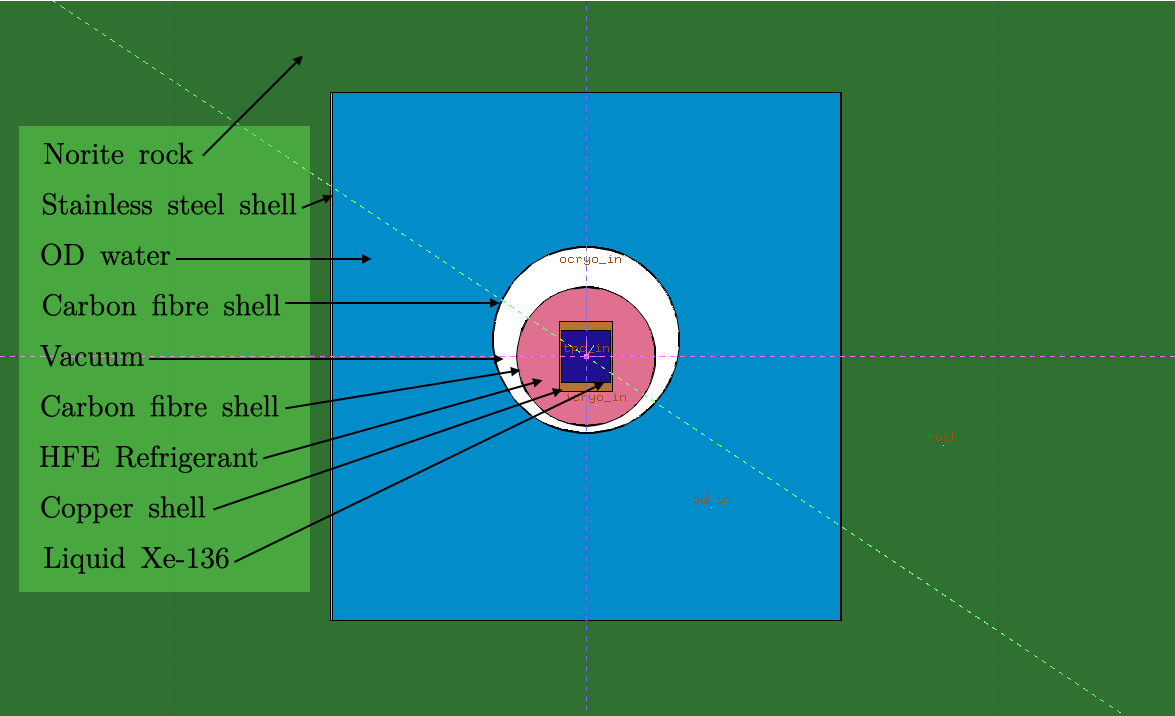
\includegraphics[scale=0.3]{figures/geometry_3.png}
    \caption{A 2D projection of the nEXO geometry used in the FLUKA simulations}
    \label{fig:geometry3}
    \end{center}
\end{figure}

\subsection{Media}
\paragraph{}
After \textit{geometry} the most natural section to discuss in the input card is the \textit{Media} section. In this section, materials are defined if they aren't in the FLUKA default material database and they're assigned to regions. There are four main types of cards in this section: \textcolor{Maroon}{MATERIAL}, \textcolor{Maroon}{COMPOUND}, \textcolor{Maroon}{ASSIGNMA}, and \textcolor{Maroon}{LOW-MAT}. 

\begin{figure}[h]
    \begin{center}
    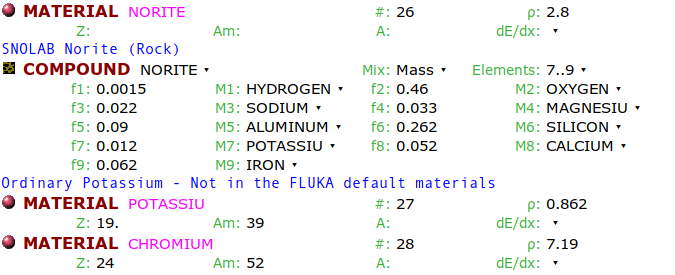
\includegraphics[scale=0.5]{figures/media_1.png}
    \caption{A subset of the media section in the input file}
    \label{fig:media1}
    \end{center}
\end{figure}

\paragraph{}
First, referring to figure \ref{fig:media1} and describe the first card in the media section. It is a \textcolor{Maroon}{MATERIAL} card with variable name \textcolor{magenta}{NORITE}. This card declares a new material called \textcolor{magenta}{NORITE} which is given a density, and a user-chosen material number for later reference \footnote{The numbers for user-defined materials can't start at 1, they proceed from the last number of the native FLUKA materials list (25)}. Norite rock is an abundant rock around the Sudbury basin. It is a mixture of various elements and must therefore be defined with the subsequent \textcolor{magenta}{COMPOUND} card. The arguments for this card are the component materials of the compound and their respective fractions by mass, volume, or atom abundance. These arguments should be very clear, the odd one out is \textcolor{ForestGreen}{Elements} which simply allows for the resizing of the compound card to accomodate more or fewer elements. The following cards, \textcolor{magenta}{POTASSIU} and \textcolor{magenta}{CHROMIUM} are necessary to define as they are not in the default FLUKA materials list. Given that these are elemental, we must provide the arguments of atomic number (\textcolor{ForestGreen}{Z}), the atomic mass (\textcolor{ForestGreen}{Am}) in g/mol, and the atomic mass number (\textcolor{ForestGreen}{A}) which is assumed to be the most abundant for the given (\textcolor{ForestGreen}{Z}) if left unspecified. Of course \textcolor{ForestGreen}{$\rho$} is the density, and \textcolor{ForestGreen}{$dE/dx$} allows to select another material to use for the case of ionization— we do not use this feature.

\paragraph{}
Once all the materials are defined they are then assigned to regions with the \textcolor{Maroon}{ASSIGNMA} cards. This card a list of arguments including the material to be assigned and the regions it will be assigned to. One of these cards can assign a material to several regions, however, the regions had to have been declared in some regular order for this to work for multiple regions. That is, a user might wish to have every region from the first to last of N regions to be full of water. In this case, the card would have arguments \textcolor{ForestGreen}{Reg:} $=$ 1 and \textcolor{ForestGreen}{to Reg:} $= N$. Alternatively, a user can assign a material to every $k^{\text{th}}$ region in the range $[1,N]$ by setting \textcolor{ForestGreen}{Step:} $=$ 3. This seems like a strange and uncomfortable way to do things because any modification to the region declarations can totally offset the material assignments. Nevertheless, it is how it works. In the ``nEXO\_OD.inp'' input file, each region is assigned a material separately and by name. This issue ought not occur.

\subsubsection{Specific Materials}
\paragraph{}
Now that the input options have been discussed, we will overview some of the materials used in the ``nEXO\_OD.inp'' input file as these may not be an exact representation of the material structure of nEXO. First, 





\part*{The Muon Source User Routine}

\part*{The Scoring User Routine (`mgdraw.f')}

\part*{Containerization with Singularity}

\part*{Interpreting Output}

% \clearpage
% % \appendixheaderon
% % \appendixpage
% % \begin{appendices}
    

% % \end{appendices}


% \newpage

% \section*{Acknowledgements}
% \paragraph{}


% \bibliographystyle{aip}
% \bibliography{manual.bib}

\end{document}